\chapter{Diskrete Symmetrien und Erhaltungssätze}
\section{Diskrete Symmetrien}
\begin{figure}[h!]
	\centering
	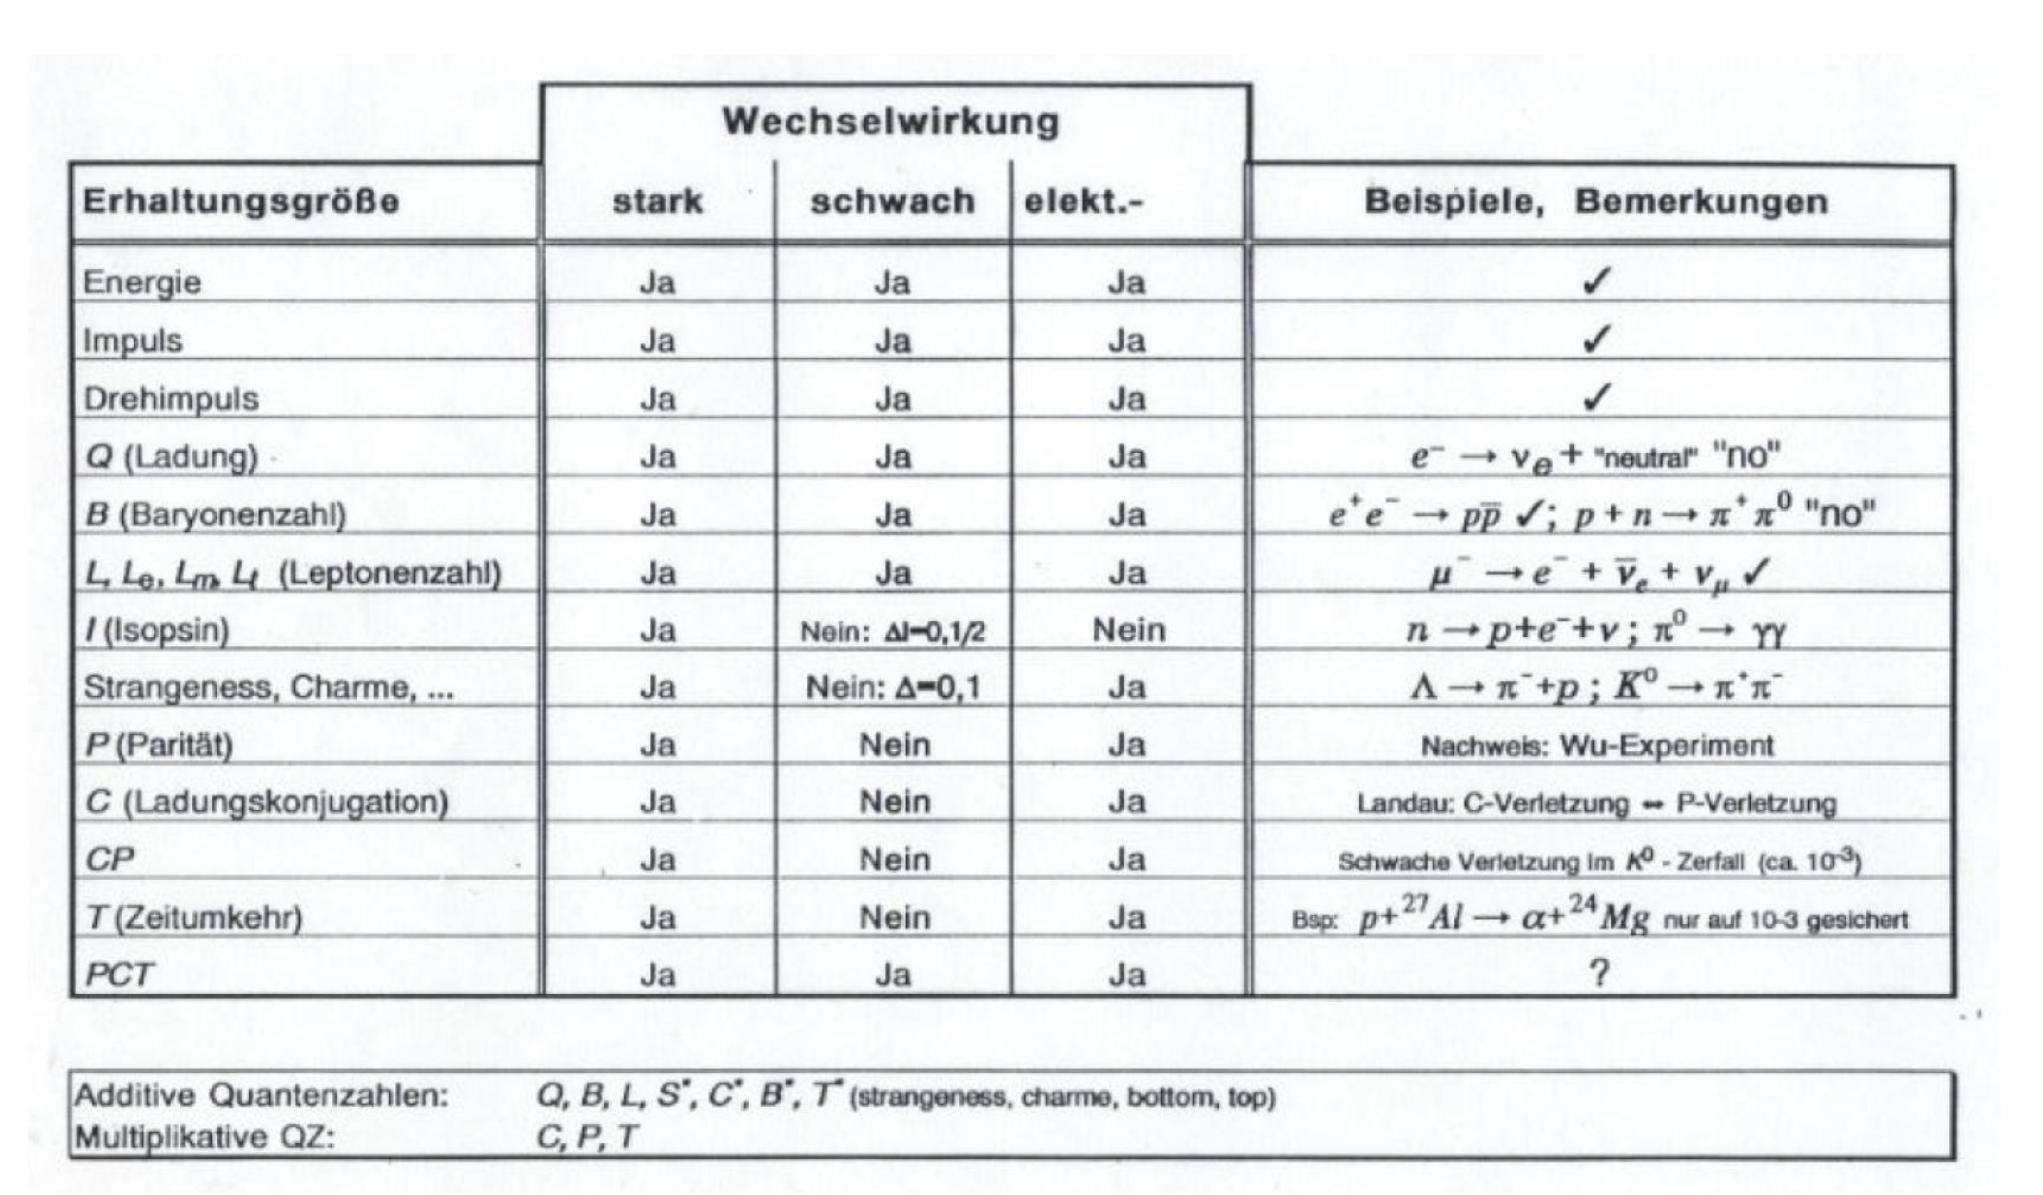
\includegraphics[width=.7\textwidth]{./img/symmetries.jpg}
	\caption{Zusammenfassung der Erhaltungsgrößen}
	\label{fig:symmetries}
\end{figure}

\section{Parität}
\subsection{Der $\mathcal{P}$-Operator}
Der Paritätsoperator $P$ erzeugt eine räumliche Spiegelung im Ursprung.
Sie ist eine mulitplikative Quantenzahl mit den möglichen Eigenwerten $\pm 1$.
Eine Reaktion $a+b\longrightarrow c+d$ hätte die Gesamtparität
\begin{equation*}
	P_a\cdot P_b\cdot (-1)^l = P_c\cdot P_d\cdot (-1)^{l'}
\end{equation*}
mit etwaigen Bahndrehimpulsen $l,l'$.
Dabei sind $P_i$ die \textbf{Eigenparitäten} der Teilchen.
Man definiert:
\begin{align*}
	P(q) &= -P(\bar{q}) = 1 \\
	P(p) &= P(n) = P(\Lambda) = 1
\end{align*}
Außerdem haben bei \textbf{Fermionen} Teilchen und Antiteilchen \textbf{entgegengesetzte} Parität,
bei \textbf{Bosonen} jedoch \textbf{gleiche} Parität.

Alle anderen Paritäten lassen sich daraus ableiten.

\subsection{Paritätsverletzung durch die schwache Wechselwirkung}
Eine einzigartige Eigenschaft der schwachen Wechselwirkung ist die, paritätsverletzend zu sein.
Reaktionen der schwachen Wechselwirkung sind nicht spiegelsymmetrisch.
Dies folgt aus der experimentell belegten Tatsache, dass die schwache Wechselwirkung eine Wechselwirkung mit Axial- und Vektorcharakter zugleich ist.
Die Stärke der Axialvektor- und Vektoranteile werden dabei durch zwei Koeffizienten $c_\text{A}$ und $c_\text{V}$ beschrieben.
Bei einer V+A-Wechselwirkung ($c_\text{V}=c_\text{A}$) koppelt die Wechselwirkung nur an rechtshändige Fermionen und linkshändige Antifermionen.
Bei einer V-A-Wechselwirkung ($c_\text{V}=-c_\text{A}$) koppelt die Wechselwirkung nur an linkshändige Fermionen und rechtshändige Antifermionen.
Für die Kopplungsstärke der W-Bosonen findet man $c_\text{V}=-c_\text{A}=1$.
Man spricht daher auch von einer V-A-Theorie der geladenen Ströme.
Die Parität ist \textbf{maximal verletzt}, wenn gilt: $|c_\text{V}|=|c_\text{A}|$, was bei geladenen Strömen zutrifft.

\begin{figure}
	\centering
	\includegraphics[width=.5\textwidth]{./img/myondecay.pdf}
	\caption{Myonzerfall, eine Möglichkeit ist unterdrückt}
	\label{fig:myondecay}
\end{figure}
Ein Beispiel für die Paritätsverletzung der schwachen Wechselwirkung ist der Myonzerfall $\mu^-\rightarrow\el + \nu_\mu + \bar{\nu}_e$ (\autoref{fig:myondecay}).
Im Ruhesystem des Myons hat das Elektron den größten Impuls, wenn die Impulse der Neutrinos parallel zueinander und entgegengesetzt zur Impulsrichtung des Elektrons stehen.
Da sich die Spins des $\nu\bar{\nu}$-Paares aufheben müssen, muss der Spin des Elektrons dem Spin des Myons gleichgerichtet sein, um Spinerhaltung zu erfüllen.
Experimentell beobachtet man, dass Elektronen aus dem Myonzerfall allerdings bevorzugt linkshändig emittiert werden!
Somit ist die Parität maximal verletzt.

\subsection{Das Wu-Experiment}
\begin{figure}
	\centering
	\begin{subfigure}{0.5\textwidth}
		\centering
		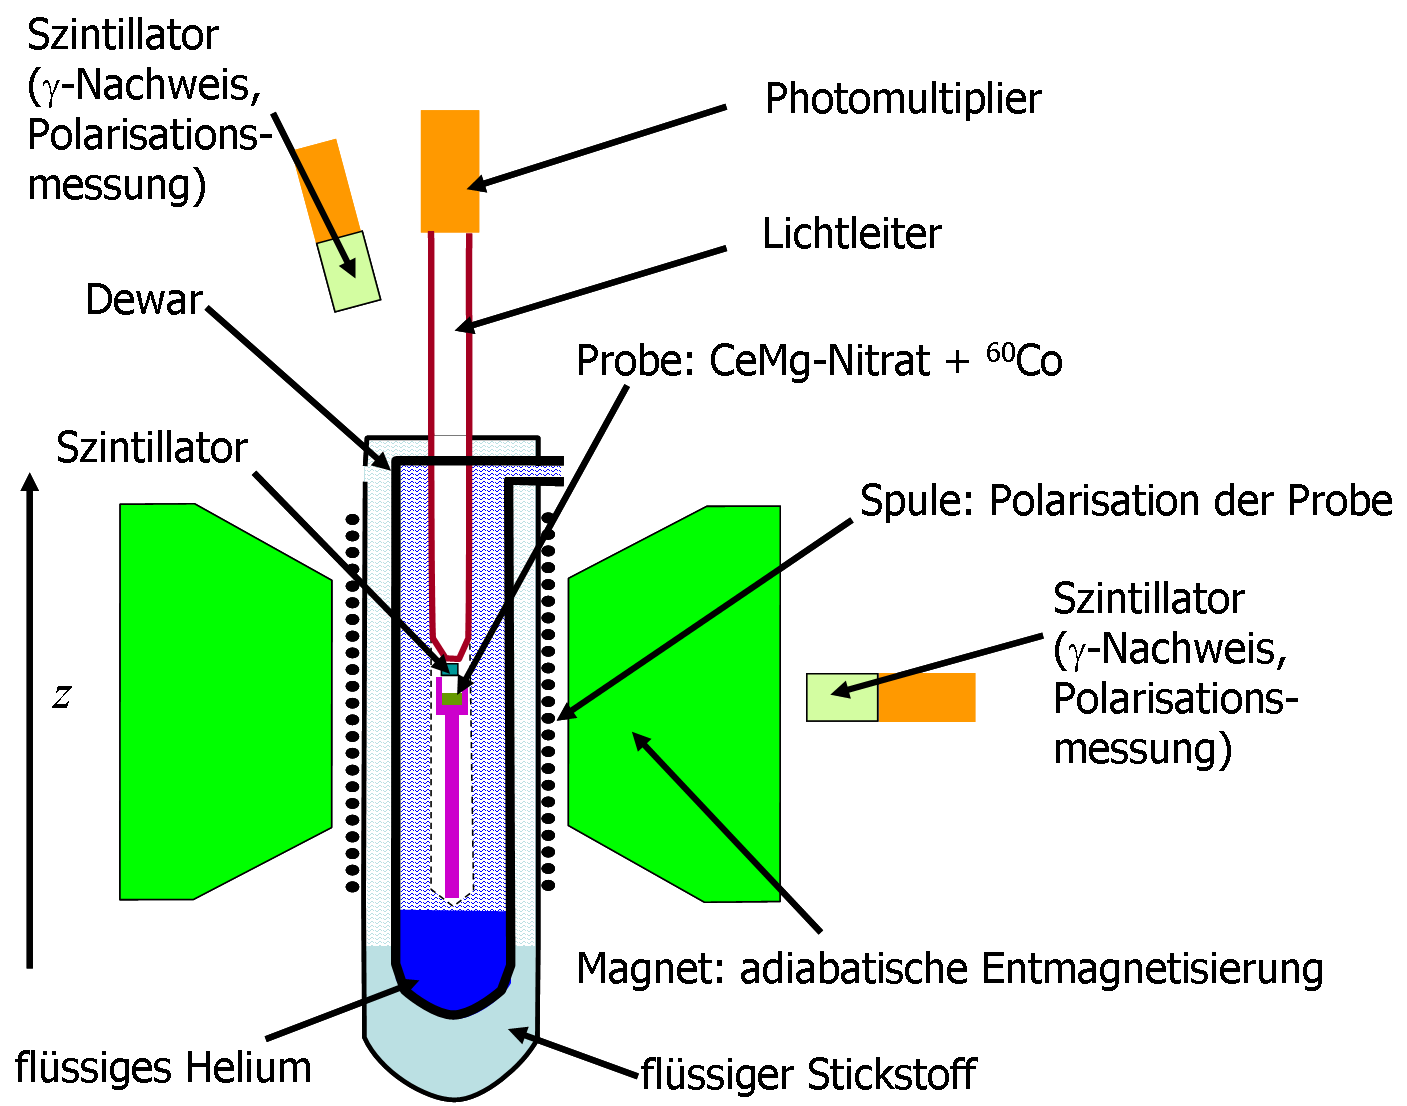
\includegraphics[width=.5\textwidth]{./img/wu.jpg}
		\caption{Das Wu-Experiment: Detektor in negativer z-Richtung}
		\label{fig:wu}
	\end{subfigure}
	\begin{subfigure}{0.4\textwidth}
		\centering
		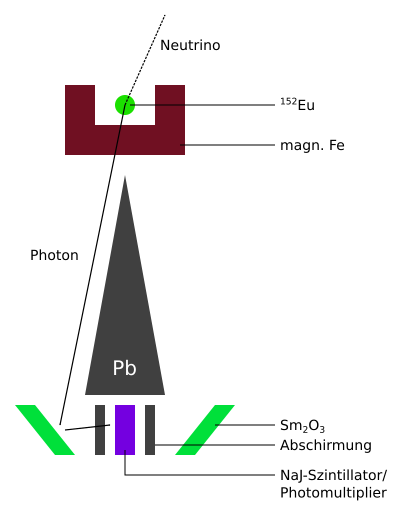
\includegraphics[width=.5\textwidth]{./img/gold.pdf}
		\caption{Das Goldhaber-Experiment: Target unten, Quelle oben}
		\label{fig:gold}
	\end{subfigure}
	\caption{Experimente zur Untersuchung der Paritätsverletzung}
\end{figure}
Eindrucksvoll konnte das Wu-Experiment die Paritätsverletzung der schwachen Wechselwirkung demonstrieren.
Es wurde der Kern-$\upbeta$-Zerfall von $^{60}Co$ untersucht.
Der Versuchsaufbau ist in \autoref{fig:wu} zu sehen.
Die Fragestellung war, ob es eine Vorzugsrichtung der beim $\upbeta$-Zerfall emittierten Elektronen relativ zum Spin des $^{60}Co$-Kerns gibt.
Die Reaktion lautet
\begin{equation*}
	Co(5+)\longrightarrow Ni^*(4+) + \el + \bar{\nu}_e.
\end{equation*}
Die technische Herausforderung dabei war, die Ausrichtung des Spins der Co-Kerne bei sehr tiefen Temperaturen.
Man verwendete das Prinzip der ’’adiabatischen Entmagnetisierung’’ ($\rightarrow$ \url{de.wikipedia.org/wiki/Magnetische_K%C3%BChlung}).

Es wird nun mit einem Detektor in negativer z-Richtung die Anzahl der emittierten Elektronen gemessen, einmal mit Magnetfeld in z-Richtung, einmal in -z-Richtung(, was einer Paritätsumkehr entspricht).
Man stellt fest, dass deutlich mehr Elektronen mit Spin antiparallel zur Spinrichtung der Kerne emittiert werden, als parallel dazu.
Dies ist die Bestätigung der maximalen Paritätsverletzung in der schwachen Wechselwirkung.

\subsection{Das Goldhaber-Experiment}
Das Goldhaber-Experiment zeigt nun sogar, dass es nur linkshändige Neutrinos und rechtshändige Antineutrinos gibt.
Betrachtet wird der Zerfall von Eu-152-Kernen in einem metastabilen Zustand durch K-Einfang
\begin{equation*}
	Eu\text{(meta)} + \el \longrightarrow Sm^* + \nu_e.
\end{equation*}
Der Tochterkern befindet sich in einem angeregten Zustand, der danach durch $\upgamma$-Emission relaxiert.
Dabei erfüllt die Zerfallskaskade folgende Eigenschaften:
\begin{itemize}
	\item Spinfolge $0^-\rightarrow 1^-\rightarrow 0^+$
	\item gleiche Übergangsenergien (ca. 1\% Abweichung der Energien)
	\item Sehr kurze Lebensdauer des Sm ($\approx\SI{3e-14}{\second}$).
\end{itemize}
\autoref{fig:gold} zeigt den Versuchsaufbau.
Der Nachweis der Gamma-Quanten aus dem Sm-Zerfall beruht auf der resonanten Streuung der Gamma-Quanten an einem Sm2O3-Target, welches ringförmig um den Detektor angebracht ist.
Die Bleiabschirmung hindert Zerfallsphotonen aus der Eu-152-Quelle daran, den Detektor direkt zu erreichen.
Die resonante Streuung findet über Kernresonanzabsorption des Photons durch einen Sm-Kern und anschließende spontane Emission statt.
Da die Quellkerne kurze Zeit zuvor ein Neutrino abgegeben haben, ist der angeregte Sm-Kern nicht in Ruhe.
Somit hat das Relaxationsphoton genügend Energie, um resonant absorbiert zu werden und der angeregte Sm-Zustand eine ausreichend geringe Lebensdauer, um nicht durch Wechselwirkungen mit dem Gitter zu relaxieren.
Dieser Trick funktioniert allerdings nur, wenn das Neutrino nach oben emittiert wurde, andernfalls ist die Energiedifferenz zu hoch.
Damit kann also die Richtung der Neutrinoemission bestimmt werden.

Durch einfache Spinbetrachtungen gelangt man zum Schluss, dass die Helizität der Relaxationsphotonen der der emittierten Neutrinos entsprechen muss.
Der Detektor wird von einem magnetisierten Eisenblock abgeschirmt, sodass etwa 7-8\% der Elektronen im Eisen polarisiert sind.
Die Compton-Streuung der Relaxationsphotonen mit den Elektronen im Eisenblock hängt stark von der Polarisierung des streuenden Materials ab.
Falls es eine Vorzugsrichtung der Helizität der Photonen und damit der Neutrinos geben sollte, so müssten sich die Zählraten je nach Magnetisierungsrichtung des Eisenblocks stark unterscheiden.
Tatsächlich misst man nur in eine Magnetisierungsrichtung Ereignisse.

Somit ist bestätigt, dass Neutrinos nur linkshändig vorkommen.

\section{Ladungskonjugation}
\subsection{Der $\mathcal{C}$-Operator}
Der C-Operator führt in einem System Teilchen in Antiteilchen und vice versa über.

\subsection{CP-Erhaltung}
Man kann leicht sehen, dass durch die festgelegte Helizität der Neutrinos die schwache Wechselwirkung C-Symmetrie von vornherein bricht (C auf linkshändiges Neutrino $\rightarrow$ linkshändiges Antineutrino, gibt's aber im SM nicht!).
Wendet man jedoch CP gemeinsam auf Prozesse an, an denen die schwache Wechselwirkung beteiligt ist, so entstehen Prozesse, die in der Natur existieren.
Die schwache Wechselwirkung ist somit CP-erhaltend.
Es gibt jedoch Fälle, bei denen die CP-Symmetrie nicht erhalten bleibt, wie zum Beispiel beim neutralen Kaonzerfall.

\subsubsection{Der Zerfall des neutralen Kaons}
\begin{figure}
	\centering
	\includegraphics[width=.5\textwidth]{./img/boxkaon.pdf}
	\caption{Boxdiagramm zur Veranschaulichung der Kaonen-Übergänge}
	\label{fig:box}
\end{figure}
Neutrale Kaonen $K^0$ können sowohl in zwei als auch in drei Pionen zerfallen.
Dabei hat das Zwei-Pion-System eine Parität von $+1$ und das Drei-Pion-System eine von $-1$.
Dies kann man sich ganz einfach daraus überlegen, dass das $K^0$ einen Gesamtdrehimpuls von 0 aufweist und die Eigenparität der Pionen $-1$ ist
\begin{equation*}
	\mathcal{P}\ket{\pi\pi} = (-1)^2\cdot (-1)^{l=0} = +\ket{\pi\pi}\qquad \mathcal{P}\ket{\pi\pi\pi} = (-1)^3\cdot (-1)^{l=0} = -\ket{\pi\pi\pi}.
\end{equation*}
Die Tatsache, dass beide Zerfälle beobachtet werden, obwohl das Kaon eine Parität von $-1$ hat, zeugt bereits von Paritätsverletzung.

Da das $K^0$ und das $\bar{K^0}$ in die gleichen Endzustände zerfallen können, können sie über einen virtuellen, pionischen Zwischenzustand mischen
\begin{equation*}
	K^0 \longleftrightarrow \twovec{2\pi}{3\pi} \longleftrightarrow \bar{K^0},
\end{equation*}
was man mit einem Boxdiagramm (\autoref{fig:box}) besser veranschaulichen kann.

Die beim Zerfall entstehenden Pion-Systeme sind Eigenzustände bezüglich des $\mathcal{CP}$-Operators
\begin{equation*}
	\mathcal{CP}\ket{\pi\pi} = +\ket{\pi\pi}\qquad\mathcal{CP}\ket{\pi\pi\pi} = -\ket{\pi\pi\pi}.
\end{equation*}
während die $K^0$ und $\bar{K^0}$ keine Eigenzustände sind
\begin{equation*}
	\mathcal{CP}\ket{K^0} = -\ket{\bar{K^0}}\qquad\mathcal{CP}\ket{\bar{K^0}} = -\ket{K^0}.
\end{equation*}

Wenn wir davon ausgehen, dass die schwache Wechselwirkung CP-erhaltend ist, so muss vor dem Zerfall ein Eigenzustand bezüglich des $\mathcal{CP}$-Operators vorgelegen haben.
Diese Zustände lassen sich konstruieren
\begin{align*}
	\ket{K^0_1} &= \frac{1}{\sqrt{2}}\left(\ket{K^0}-\ket{\bar{K^0}}\right) \quad\text{mit}\ \mathcal{CP}\ket{K^0_1} = +\ket{K^0_1} \\
	\ket{K^0_2} &= \frac{1}{\sqrt{2}}\left(\ket{K^0}+\ket{\bar{K^0}}\right) \quad\text{mit}\ \mathcal{CP}\ket{K^0_2} = -\ket{K^0_2}.
\end{align*}
Nach diesen Überlegungen sollte der $\ket{K^0_1}$-Zustand aufgrund von CP-Erhaltung also in zwei Pionen und der $\ket{K^0_2}$-Zustand in 3 Pionen zerfallen.
Da der Phasenraum für 3-Körperzerfälle erheblich kleiner ist als für einen 2-Körperzerfall, sollte demnach das $\ket{K^0_2}$ auch deutlich langlebiger sein als das $\ket{K^0_1}$.
In der Tat beobachtet man bei Reaktionen, in denen neutrale Kaonen entstehen, eine Mischung von kurz- und langlebigen Teilchen, die man als $K^0_\text{L}$ und $K^0_\text{S}$ bezeichnet.

Dieses Mischungsverhältnis von anfangs 50:50 ändert sich mit der Zeit.
Die Zeitentwicklung von $K^0$ und $\bar{K^0}$ zeigt ein typisches Oszillationsverhalten, wie man es für ein quantenmechanisches System aus zwei Basiszuständen kennt.
Man nennt diese Oszillation \textbf{Strangeness-Oszillation}.

Will man einen reinen $K^0_\text{L}$-Strahl haben, so baut man seinen Detektor in einiger Entfernung von der $K^0$-Quelle auf, sodass die $K^0_\text{S}$ bis dahin bereits zerfallen sind und nur noch die $K^0_\text{L}$ übrig sind.
Daraus kann man aber auch wieder einen gemischten Strahl herstellen, indem man einfach ein Stück Materie in den Strahlgang bringt.
Da der $K^0_\text{L}$-Strahl zu 50:50 $K^0$ und $\bar{K^0}$ enthält, werden die Antiteilchen stärker im Material absorbiert und man erhält überwiegend einen Strahl aus $K^0$, welcher ja wieder $K^0_\text{S}$ enthält.

Betrachten wir nun ein Experiment, in dem genau dieser Versuchsaufbau vorliegt.
Ein Detektor wurde so weit von der Quelle platziert, sodass wir einen reinen $K^0_\text{L}$-Strahl haben.
Wenn CP-Erhaltung gilt, dürften wir also nur 3-Pionzerfälle beobachten.
Dieses Experiment wurde im Jahr 1964 durchgeführt und es wurde erstmals nachgewiesen, dass das $K^0_\text{L}$ auch mit einer geringen Wahrscheinlichkeit in 2 Pionen zerfällt, was der erste Nachweis für eine CP-Verletzung war.

Man führt dies darauf zurück, dass der Masseneigenzustand $K^0_\text{L}$ nicht identisch mit dem CP-Eigenzustand $K^0_1$ ist, sondern wiederum eine Mischung aus $K^0_1$ und $K^0_2$ mit einem komplexen Mischungsparameter $\epsilon$, welcher die beiden Zustände gewichtet.
